%\documentclass[conference]{IEEEtran}
\documentclass[10pt, conference, letterpaper]{IEEEtran}
%% INFOCOM 2013 addition:
\makeatletter
\def\ps@headings{%
\def\@oddhead{\mbox{}\scriptsize\rightmark \hfil \thepage}%
\def\@evenhead{\scriptsize\thepage \hfil \leftmark\mbox{}}%
\def\@oddfoot{}%
\def\@evenfoot{}}
\makeatother
\pagestyle{headings}

\usepackage{amsmath}
\usepackage{algorithm}
\usepackage{algorithmic}
\usepackage{graphicx}
\usepackage{cite}
%\usepackage{mathrsfs}
\usepackage[bookmarks=false]{hyperref}
\usepackage{array}
\usepackage{cases}
\usepackage{booktabs}
\usepackage{multirow}
\usepackage{threeparttable}


%
%\begin{flushleft}\fontsize{8.5pt}{0.6\baselineskip}\selectfont{Remarks: 1) ``$-$" means the algorithm is not applicable to
%oblivious blind rendezvous; 2) ETTR means expected time to rendezvous (note: MMC cannot guarantee rendezvous in bounded time); 3) $P$ is the smallest prime number larger than $N$, $P=O(N)$. 4) $k_a$ and $k_b$ denote the numbers of two users' available channels; 5) SCH in this paper is only suitable for synchronous users.
%}\end{flushleft}


\newtheorem{property}{Property}[section]
\newtheorem{theorem}{Theorem}
\newtheorem{lemma}{Lemma}[section]
\newtheorem{claim}[lemma]{Claim}
\newtheorem{remark}{Remark}[section]
\newtheorem{definition}{Definition}[section]
\newtheorem{corollary}{Corollary}
\newtheorem{problem}{Problem}

\ifCLASSINFOpdf

\else

\fi

\ifCLASSOPTIONcompsoc
\usepackage[tight,normalsize,sf,SF]{subfigure}
\else
\usepackage[tight,footnotesize]{subfigure}
\fi

% correct bad hyphenation here
\hyphenation{op-tical net-works semi-conduc-tor}


\begin{document}


\bibliographystyle{plain}

\title{How Local Information Improves Rendezvous in Cognitive Radio Networks}

%\author{\IEEEauthorblockN{
%Zhaoquan Gu\IEEEauthorrefmark{1}, Haosen Pu\IEEEauthorrefmark{1}, Qiang-Sheng Hua\IEEEauthorrefmark{2}, and
%Francis C.M. Lau\IEEEauthorrefmark{3}}
%
%\IEEEauthorblockA{\IEEEauthorrefmark{1}Institute for Interdisciplinary Information Sciences, Tsinghua University,
%Beijing, China\\}
%\IEEEauthorblockA{\IEEEauthorrefmark{2}School of Computer Science $\&$ Technology, Huazhong University of Science and Technology, China\\}
%\IEEEauthorblockA{\IEEEauthorrefmark{3}Department of Computer Science, The University of Hong Kong, Hong Kong, China\\}
%}

\maketitle


\begin{abstract}
Cognitive Radio Network (CRN) is a promising technique aiming at solving the wireless spectrum scarcity problem. Rendezvous is the fundamental process of CRN.  We are devoted to design faster rendezvous algorithms for CRN. We find that local information such as user's ID and the label of an available channel is very useful for designing faster rendezvous algorithms. First, we propose an Asynchronous  Anonymous Non-oblivious Global-channel-based (AANG) algorithm. AANG algorithm can guarantee rendezvous for any two users $i,j$ in $2P^2+2P$ timeslots, where $P$ is the least prime not less than the total number of channels in the network. Second, we utilize the user's identifier (ID) to design an Asynchronous Non-anonymous Oblivious Local-channel-based (ANOL) algorithm. ANOL algorithm can guarantee rendezvous for any two users $i$ and $j$ in $(l+1)(P_i+2)(P_j+2)$ timeslots, where $P_i$ and $P_j$ are the smallest primes which are not less than the numbers of available channels of user $i$ and $j$ respectively. Third, we propose an Asynchronous Anonymous Non-obvious Local-sequence-based (AANL) rendezvous algorithm which can guarantee rendezvous for any two users in $((P_i +2)(P_j+2) + P)(\left \lceil log_2 N \right \rceil + 1)$ timeslots, where $N$ is the overall amount of channels in the network and $P$ is the least prime which is not less than $N$.  All of our algorithms can be used in multi-user scenario. We conduct plenty of experiments comparing our algorithms with state-of-the-art rendezvous algorithms under different scenarios, which corroborate our analysis.
\end{abstract}


\begin{IEEEkeywords}
Cognitive Radio Network, Local Information, Rendezvous Algorithms, Channel Label, identifier
\end{IEEEkeywords}

\section{Introduction}
The wireless spectrum is invaluable for the transmission of wireless signals because the resource of wireless spectrum is finite. The wireless spectrum is divided into licensed spectrums and unlicensed spectrums. However, the overcrowding problem of the unlicensed spectrums is becoming more and more severe due to the rapid growth of wireless devices. On the other hand, the utilization rate of the licensed spectrums is relatively low. Cognitive Radio Network (CRN) is a promising solution for this problem. In CRN, there exist two kinds of users, primary users (PUs) and secondary users (SUs). A PU owns one or more licensed channels while a SU needs to search for ``empty" licensed spectrums which are not occupied by PUs \footnote{Unless specifically pointed out, ``users" in the rest of this paper refer to SUs.} to complete communication task.

CRN contains many important stages such as broadcasting, routing, data gathering, neighbor discovery and so on. \emph{Rendezvous} is the fundamental task of CRN, which targets finding a common frequency band (channel) for different users to communicate on. Before rendezvous completes, a user may even not aware of the existence of another user, let alone exchange information.


To achieve rendezvous between users, many solutions have been proposed. Some works requires a central controller or a common control channel (CCC) to achieve rendezvous. However, it is not practical to establish a central controller to control all the users in large-scale networks. And if the number of users exceeds the capacity of the central controller or CCC, this method will become invalid. And it is not safe from the perspective of information security, for the probability of adversary attacks. Hence, some researchers proposed some algorithms without central controller or CCC, which are called blind rendezvous algorithms. Blind rendezvous algorithms are more practical than CCC based rendezvous algorithms. Channel Hopping (CH) technique is widely used in blind rendezvous algorithms. In CH algorithms, users hop to channels according to predefined sequences.

\begin{table*}[!t]
\renewcommand{\arraystretch}{1.3}
 \caption{\upshape Comparisons between rendezvous algorithms }
\centering
\begin{tabular}{|c|c|c|c|c|c|c|c|}
\hline
\multirow{2}*{Algorithm} &  \multirow{2}*{MTTR} & \multirow{2}*{RD} & \multirow{2}*{Time} & Anonymous or & Oblivious or &\multirow{2}*{Sequence}& Single Radio\\
 & & &  & Non-Anonymous & Non-Oblivious & & or Multi-radio\\
 \hline
JS & 3NP(P-G) +3P & 100\% & Asynchronous & Anonymous & Non-Oblivious & Global & Single-radio\\
\hline
DRDS & $3P^2 + 2P$ & 100\% & Asynchronous & Anonymous & Non-Oblivious & Global & Single-radio\\
\hline
CBH & $2l_pP^2$ & 100\% & Asynchronous & Non-Anonymou & Oblivious & Local & Single-radio\\
\hline
HH & $3|C_a||C_b|$ &$ 100\%$ & Asynchronous & Anonymous & Non-Oblivious & Local & Single-radio\\
\hline


Adv.rdv-$l$ & $(g+log_2g)P_iP_j$ & 100\% & Asynchronous & Non-Anonymous & Oblivious & Local & Single-radio\\
\hline

Adv.rdv-$\eta_1$ & $(2g+3)P_iP_j$ & 100\% & Asynchronous & Non-Anonymous & Oblivious & Local & Single-radio\\

\hline
%(g+\left \lceil \sqrt{g} \right \rceil (2 + \left \lceil log_2g \right \rceil)
\multirow{2}*{Adv.rdv-$\eta_2$ }&  $(g+\left \lceil \sqrt{g} \right \rceil (2 $ & \multirow{2}*{100\%} & \multirow{2}*{Asynchronous} & \multirow{2}*{Non-Anonymous} & \multirow{2}*{Oblivious} & \multirow{2}*{Local} & \multirow{2}*{Single-radio}\\
 & $+ \left \lceil log_2g \right \rceil)P_iP_j$ &  & & & & & \\
 \hline

% GCR & $max\{p_i,p_i'\}max\{p_j,p_j'\}$ &  100\% & Asynchronous & Anonymous & Oblivious & Local & Two-radio\\
% \hline
%
%\multirow{2}*{AMRR} & $max\{|V_1|,|V_2|\}$ & \multirow{2}*{100\%} & \multirow{2}*{Asynchronous} & \multirow{2}*{Anonymous} & \multirow{2}*{Oblivious} & \multirow{2}*{Local} & \multirow{2}*{Multi-radio} \\
% & $\times (max\{|V_1|,|V_2|\}+1) $  & & & & & & \\
%\hline

\multirow{2}*{MTP} & $2(max\{m_a,m_b\})^2$ & \multirow{2}*{100\%}& \multirow{2}*{Asynchronous}  & \multirow{2}*{Anonymous} & \multirow{2}*{Oblivious} & \multirow{2}*{Local} & \multirow{2}*{Multi-radio}\\
 & $\times 32(\left \lceil loglog \; n \right \rceil + 1)$ & & & & & & \\
\hline

AANG(this paper) & $2P^2 + 2P$ & $<100\%$ & Asynchronous & Anonymous & Oblivious & Global & Single-radio\\
\hline
ANOL(this paper) & $(l  + 1)(P_i + 2)(P_j + 2)$ & 100\% &Asynchronous & Non-Anonymous & Oblivious & Local & Single-radio\\
\hline
%ANOL(this paper) & $3(P_i+1)(P_j+1)(\left \lceil log_2N \right \rceil +1)$ & $<100\%$ &Asynchronous & Non-Anonymous & Oblivious & Local & Single-radio\\
%\hline

\multirow{2}*{ANOL(this paper)} & $((P_i +2)(P_j+2) + P)$ & \multirow{2}*{$<100\%$}& \multirow{2}*{Asynchronous}  & \multirow{2}*{Anonymous} & \multirow{2}*{Oblivious} & \multirow{2}*{Local} & \multirow{2}*{Single-radio}\\
 & $\times (\left \lceil log_2N \right \rceil +1)$ & & & & & & \\
\hline
%SSH(this paper) & $N$ & 100\% & semi-synchronous &$\times$ &$\times $ & $\times$ \\
%\hline
\end{tabular}
\end{table*}

Existing blind rendezvous algorithms can be categorized into different categories as follows.

\bfseries (i) Synchronous/asynchronous algorithms. \mdseries  Synchronous algorithms suppose there exists a global clock and every user in the network starts rendezvous process at the same time. Asynchronous algorithms don't require a global clock and every user can start rendezvous process at any time.

\bfseries (ii) Anonoymous/non-anonymous algorithms. \mdseries Anonymous algorithms don't require every user to have a unique ID. Non-anonymous algorithms suppose there exists a unique identifer (ID) for every user and take use of a user's ID to generate the channel hopping sequence.

\bfseries (iii) Oblivious/non-oblivious algorithms. \mdseries Oblivious algorithms don't require there exists a global labeling of all the channels and every user labels channels in the same way. Non-oblivious algorithms require global labeling of channels and leverages it to guarantee rendezvous.

\bfseries (iv) Global-sequence-based/local-sequence-based algorithms. \mdseries Global-sequence-based algorithms construct channel hopping sequences containing all the channels. If a channel is not in the available channel set of a user, replace it with one available channel.
Local-sequence-based algorithms generates channel hopping sequences utilizing only the local available channels as if a user is not aware of the existence of other channels.

\bfseries (v) Single-radio/multi-radio algorithms. \mdseries Single-radio algorithms suppose every user in the network is equipped with only one cognitive radio. Hence, one user can once can only hop to one channel. Multi-radio algorithms assume every user in the network is equipped with more than one cognitive radios. Hence, one user can hop to one or more channels simultaneously.

Rendezvous algorithms can be judged according to some common metrics, such as \emph{Expected Time To Rendezvous (ETTR)}, \emph{Maximum Time To Rendezvous (MTTR)}, \emph{Average Time To Rendezvous (ATTR)}, \emph{Rendezvous Degree (RD)}. \emph{Time To Rendezvous (TTR)} is the number of timeslots consumed from the last user starts rendezvous until the completion of rendezvous. ATTR is the average TTR of an algorithm. MTTR is the maximum TTR needed to achieve rendezvous. In other words, MTTR is the TTR in the worst case. It is obvious that two users can have more than one common channel, RD is the ratio of the least number of different rendezvous channels to the total number of common channels between any two users. It is obvious that the larger RD is, the more channels two users can rendezvous on. Because a channel can be not accessible to a user for some reasons, a larger ID can increase the probability of rendezvous between users. In other words, the larger RD is, the better.

In this paper, we introduce some simple but time-efficient rendezvous algorithms under different scenarios. The following are the main contributions of our paper:
\begin{itemize}
\item[1)] We propose a non-anonymous local-sequence-based rendezvous algorithm which outperforms state-of-the-art non-anonymous local-sequence-based rendezvous algorithms.
\item[2)] We propose a two-radio local-sequence-based rendezvous algorithm which outperforms the state-of-the-art two-radio local-sequence-based rendezvous algorithm.
\item[3)] We formulate the concept of semi-synchronous model and propose a semi-synchronous global-sequence-based rendezvous algorithm which is feasible and has a MTTR of $N$, which is least in all the existing rendezvous algorithms.
\item[4)] We conduct lots of experiments to compare our algorithms with state-of-the-art algorithms. The results show that our algorithms outperforms state-of-the-art rendezvous algorithms.
\end{itemize}


The rest of this paper is organized as follows. Section \uppercase\expandafter{\romannumeral2} introduces the background and some related works. Section \uppercase\expandafter{\romannumeral3} introduces different categories of models for rendezvous problem and problem formulation. Section \uppercase\expandafter{\romannumeral4} presents a non-anonymous local-sequence-based rendezvous algorithm and analyzes its performance. Section \uppercase\expandafter{\romannumeral5} presents a two-radio local-sequence-based rendezvous algorithm and analyzes its performance. Section \uppercase\expandafter{\romannumeral6} presents a semi-synchronous global-sequence-based rendezvous algorithm and analyzes its performance. Simulation results are displayed in Section Section \uppercase\expandafter{\romannumeral7}. And we conclude this paper in Section \uppercase\expandafter{\romannumeral8}.




\section{Background and Related Works}


\subsection{Prime number and Co-prime Numbers}
Prime number is a very important concept in number theory. We first introduce the definition of prime number:
\begin{definition}
A prime number is a natural number which is larger than 1 and can be divided with no remainder only by 1 and itself.
\end{definition}

The smallest prime number is 2. There is an important theory about prime number:
\begin{theorem}
If n is a positive integer and $n \ge 2$, there must exists at least one prime number between n and 2n.
\end{theorem}

Then we introduce the definition of composite number:
\begin{definition}
A composite number is a natural number which is larger than 1 and has factors besides 1 and itself.
\end{definition}

The smallest composite number is 4. There is a property about prime and composite numbers:

\begin{lemma}
Any positive integer larger than 1 is either a prime number or a composite number.
\end{lemma}

Then we introduce the definition of co-prime numbers:
\begin{definition}
Two nonzero natural integers a and b are said to be co-prime if the only common factor which could divide them with no remainder is 1.
\end{definition}

Co-prime numbers have many important properties:
\begin{lemma}
If a and b are co-prime, the least common multiple of them is their product: $a \times b$.
\end{lemma}
\begin{lemma}
If a and b are two consecutive positive integers, a and b are co-prime.
\end{lemma}
\begin{lemma}
If a and b are two consecutive positive odd numbers, a and b are co-prime.
\end{lemma}
\begin{lemma}
Suppose a is a prime number and b is a composite number. If a is larger than b, they are co-prime. If b is larger than a, but b is not a multiple of a, they are co-prime.
\end{lemma}

We then introduce an important theorem for rendezvous:
\begin{theorem}
\label{theo}
If m and n are co-prime numbers, then for any integer a, the integers $a, a + n, a + 2n,\cdots, a+(m-1)n$ are m distinct numbers under modulo-m arithmetic.
\end{theorem}
\begin{IEEEproof}
Choose any two integers from $a, a+n, a + 2n,\cdots, a+(m-1)n$, the absolute value of their difference is kn, where $0 < k < m$. If kn mod m equal 0, then $kn = lm$, where l is a positive integer. Then kn or lm is a common multiple of m and n. From Lemma 2.2 we know mn is the least common multiple of m and n, and because $0 < k < m$, kn is a common multiple of m and n that is less than mn, which is a contradiction. Hence, Theorem \ref{theo} holds.
\end{IEEEproof}

\begin{figure}[!t]
\centering
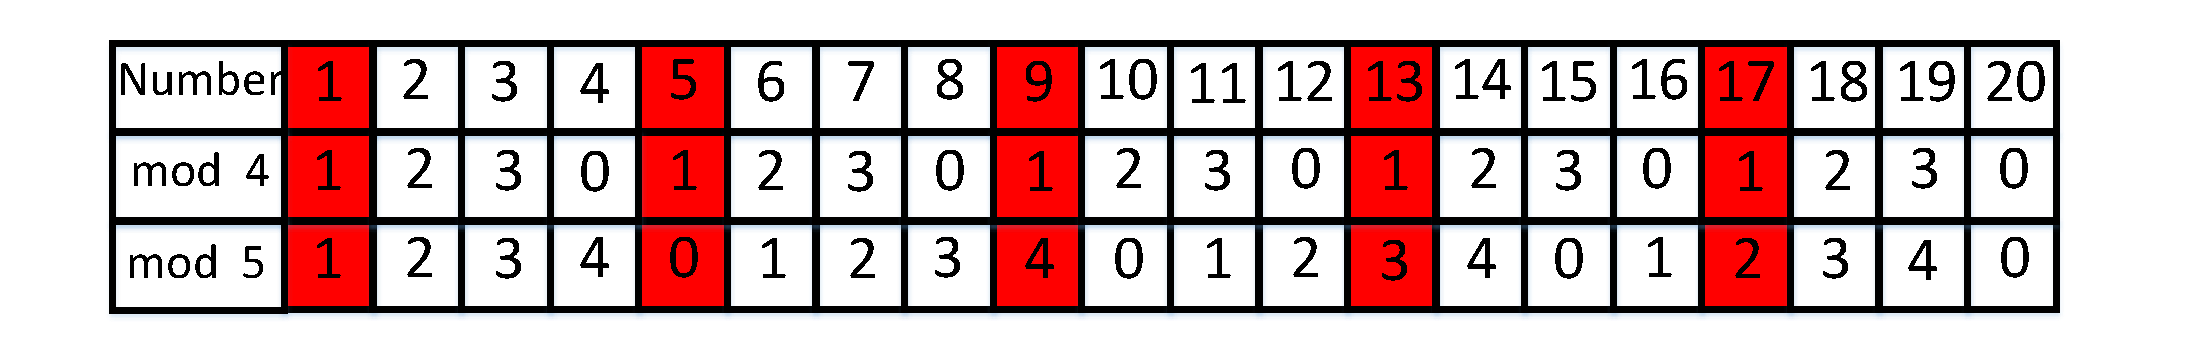
\includegraphics[width=1\columnwidth]{theo}
\caption{An example of Theorem \ref{theo}.}
\label{exp1}
\end{figure}

Fig. \ref{exp1} illustrates an example of Theorem \ref{theo}. In Fig. \ref{exp1}, the first row is a string of numbers starting from 1. The second row is the results of these numbers under modulo 4 arithmetic. The third row is the results of these numbers under modulo 5 arithmetic. We can clearly see that 1, 5, 9, 13, 17 all correspond to 1 under modulo 4 arithmetic, but correspond to 1, 0, 4, 3, 2 respectively under modulo 5 arithmetic, which are all the possible results under modulo 5 arithmetic. Theorem \ref{theo} plays an important role in rendezvous algorithms and is the main tool we use to design the following algorithms.
\subsection{Related Works}

\section{Models and Problem Formulations}
In this section, we will introduce the foundation model and some other models which are based on the foundation model. Models are of great importance in the design of rendezvous algorithms, because models constrain the resources that we can use. Hence, we need to design different algorithms under different models to achieve high performance for rendezvous process. We will also give the formulation for rendezvous problem in this section.


\subsection{Foundation Model}
Suppose there are M users in the network. Suppose the licensed spectrum is divided into n channels which are non-overlapping. Denote the set of channels as $U=\{1,2,\cdots,n\}$, where n is the total number of channels in U. We assume that every user in the network is equipped with a CRN. User i can sense a set of channels as
$C_i=\{c_{i1},c_{i2},\cdots,c_{in_i} \}$, where $n_i$ is the number of channels in set $C_i$. A channel is available to user i when it is not occupied by a PU and it is in $C_i$. User i has a set of available channels as $V_i = \{v_{i1},v_{i2},\cdots,v_{im_i}\}$, where $m_i$ is the number of channels in set $V_i$. For simplicity, we suppose that $V_i$ doesn't change during the rendezvous process. Let the length of every timeslot be 2t, where $t=10ms$ according to IEEE 802.22.

\begin{figure}
\centering
\subfigure[case 1]{
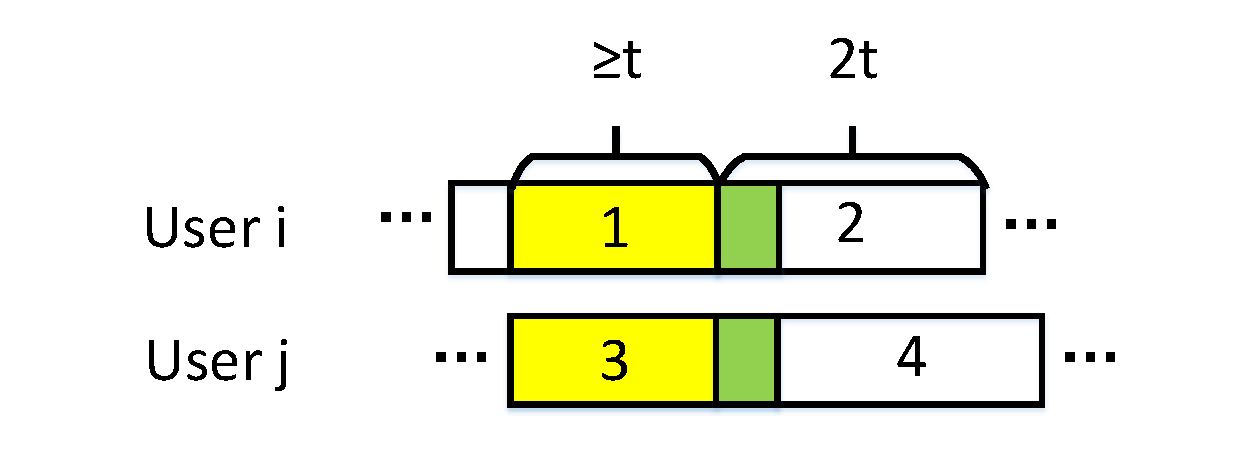
\includegraphics[width=1.6in]{olp1}
\label{olp1}
}
\subfigure[case 2]{
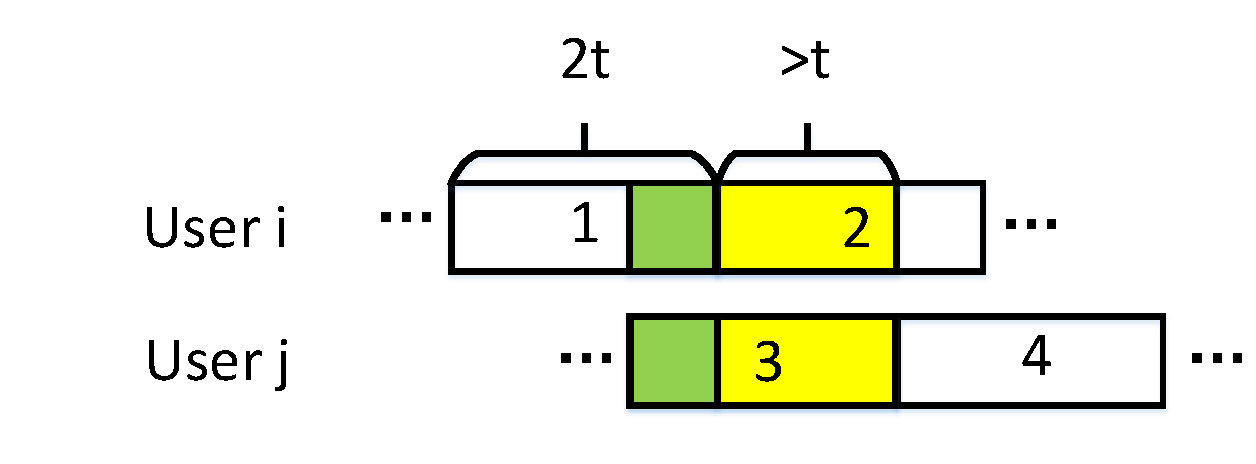
\includegraphics[width=1.6in]{olp2}
\label{olp2}
}
\caption{An example of different cases of timeslot overlapping.}
\label{overlap}
\end{figure}

Because the lengths of all users' timeslots are equal, user j's one timeslot can overlap with at most two consecutive timeslots of user i. Fig. \ref{overlap} illustrates this problem in two cases. Suppose timeslot 3 is one timeslot of user j. And the left timeslot of user i which overlaps with timeslot 3 is timeslot 1. The right timeslot of user i which overlaps with timeslot 3 is timeslot 4. The yellow part stands for the overlapping part of timeslot 1 and 3, while the green part stands for the overlapping part of timeslot 2 and 3. In Fig. \ref{olp1}, the length of the yellow part is greater than or equal to t. In Fig. \ref{olp2}, the length of the green part is greater than t.
There is a special case that the length of the yellow part or the green part is zero, which means that the timeslots of user i and user j are aligned.
Hence, no matter when the users start their rendezvous process, the maximum overlap of their timeslots is at least t, which is enough for two users to find each other and exchange information.Foundation model is the basis of other models we will introduce in the following subsections.
%
%\subsection{Oblivious and Non-Oblivious Models}
%The difference between oblivious and non-oblivious models is whether there exists a global label for every channel in $U$ and users label channels as same as their global labels. In oblivious model, there doesn't exist any global label and every user labels channels in its own way. For example, for the same channel, denote it as c, user i can label it as 1 while user j can label it as 2. In non-oblivious model, there exist global labels for channels such as $U=\{1,2,\cdots,n\}$ where we label the i-th channel in U as i. And the label of every channel for every user is as same as its global label.  It is obvious that designing rendezvous algorithms for oblivious model is at least not easier than non-oblivious model, since in non-oblivious model, we could use the labels of channels as an extra resource for designing rendezvous algorithms.

%\subsection{Anonymous and Non-Anonymous Models}
%The difference between an is whether each user in the network has a unique ID. In anonymous model, there doesn't exist a unique ID for each user. Hence, a user can't be distinguished from the other users. In non-anonymous model, there exists a unique ID for each user. Hence, a user is easily distinguishable from the other users. Designing rendezvous algorithms for non-anonymous model is easier than anonymous model, because we can use IDs, which will be shown very powerful for rendezvous process.
%
%\subsection{Synchronous, Asynchronous and Semi-Synchronous Models}
%In the previous works, there exist synchronous and asynchronous rendezvous algorithms. In synchronous model, there exists a global clock, and time is divided into equal timeslots. And every user start their rendezvous process from the same timeslot. In asynchronous model, there doesn't exist any global clock, time is divided into equal timeslots according to their local clock. And every user can start its own rendezvous process at any time.
%
%In this paper, we introduce a new model about timing, which is semi-synchronous model. In semi-synchronous model, there exists a global clock, and time is divided into equal timeslots. However, every user can start its own rendezvous process at any timeslot. Though synchronous model is difficult to implement, semi-synchronous model is practical. There exist many techniques to achieve time giving, such as GPS timing, Beidou satellite time giving, CSAO time giving and so on. These time services have high precision. For example, GPS timing can achieve 10 nanosecond level precision. Because our timeslot is 20 ms long, this level of precision is enough for our use.
%
%We need to point out that different models in different subsections can be combined to generate a new model. We will propose some algorithms for three combined models.

\subsection{Problem Formulations}
In this paper, we focus on designing rendezvous algorithms for two-user scenario, because it is the fundamental process for multiple-user rendezvous. Two-user rendezvous algorithms can be expanded into multiple-user rendezvous algorithms. Then we give the formulations of the three problems we will solve:
\begin{problem}
Utilize an arbitrary available channel of a user to design an asynchronous anonymous non-oblivious global-sequence-based rendezvous algorithm which has low MTTR and high RD.
\end{problem}

\begin{problem}
Utilize the ID of a user to design an asynchronous non-anonymous oblivious local-sequence-based rendezvous algorithm which has low MTTR and highest RD.
\end{problem}

\begin{problem}
Utilize an arbitrary available channel of a user to design an asynchronous anonymous non-oblivious local-sequence-based rendezvous algorithm which has low MTTR and high RD.
\end{problem}

\section{A Global-sequence-based Rendezvous Algorithm Based on the Channel Label}

In this section, we will propose a global-sequence-based rendezvous algorithm which is based on the channel label.

We first propose an algorithm to generate the subsequences to be used.

\begin{algorithm}
\caption{Subsequence Generating Algorithm}
\label{alg2}
\begin{algorithmic}[1]
\STATE Input: the set of available channels $V=\{v_1,v_2,\cdots,v_m\}$, and length $L$;
\STATE Initialize array $S$ with length $L$;
\STATE Initialize $i :=0$;
\WHILE {$i < L$}
\IF{$i \le m$}
\STATE $S[i] := v_i$;
\ELSE
\STATE Randomly choose a channel from $V$, denote it as $c$;
\STATE $S[i] := c$;
\ENDIF
\STATE $i:=i+1;$
\ENDWHILE
\STATE Output: Sequence $S$.
\end{algorithmic}
\end{algorithm}

The main idea of Alg.\ref{alg2} is to generate a subsequence $S$ with length $L$ according to $V$. The process is rather simple. We fill the first $m$ elements in $S$ with the channels in $V$. For the rest $(L-m)$ elements, we randomly pick channels from $V$ to fill them.


\begin{algorithm}
\caption{Global-Sequence-Based Non-Oblivious Rendezvous Algorithm}
\label{alg1}
\begin{algorithmic}[1]
\STATE Input: the set of available channels $V=\{v_1, v_2, \cdots, v_m\}$ and the total number $N$ of all channels;
\STATE Find the least prime $P$ that ensure $P \ge N$;
\STATE Randomly choose a channel from $V$, denote it as channel ($c$);
\STATE Initialize $t := 0$;
\WHILE {$0 \le t < 2P$}
\STATE Access channel ($c$);
\STATE $t:=t+1$;
\ENDWHILE
\STATE Invoke Alg.\ref{alg2} to generate a subsequence $S$ with channel set $V$ and length $P$;
\WHILE {Not rendezvous}
\IF{$t \ne 2P$ and $t $ mod $ (2P) = 0$}
\STATE Rotate $S$ to the right by $c$ steps;
\ENDIF
\STATE Access channel $S[t$ mod $P]$;
\STATE $t := t + 1$
\ENDWHILE

\end{algorithmic}
\end{algorithm}




In Alg. \ref{alg1}, we first find the least prime which is not less than the total number of  all channels. Then we randomly choose a channel from $V$, denote it as channel ($c$), and access this channel for the first $2P$ timeslots. We call this the \bfseries first stage \mdseries, the following is the \bfseries second stage \mdseries.

Then, we will generate a subsequence $S$ with length $P$. If channel $(a)$ is in the available channel set $V$, the $a-th$ channel in $S$ is channel $(a)$. For the channels that are not exist in $V$, their places will be replaced by channels which are randomly picked from $V$. And the last $(P-n)$ channels in $S$ are randomly picked from $V$. The period is $2P$ timeslots. Then we will rotate the sequence by $c$ steps to the right every period. In every period, we will hop to channels according to rotated sequence.

Fig.\ref{seq1} illustrates an example of the original generated subsequence and the first rotated subsequence. In this example, $V =\{1,3,5,6\}$ and $n=6$, so $P=7$. We generate a sequence as Fig.\ref{sq1}, where the blue rectangles correspond to randomly picked channels. And a rectangle with number in it, denote it as $i$,  represents the Channel ($i$). Because the least label in $V$ is 1, so the sequence is rotated by 1 step to the right every period. The first rotated sequence is shown in Fig.\ref{sq2}.

\begin{figure}
\centering
\subfigure[Original subsequence]{
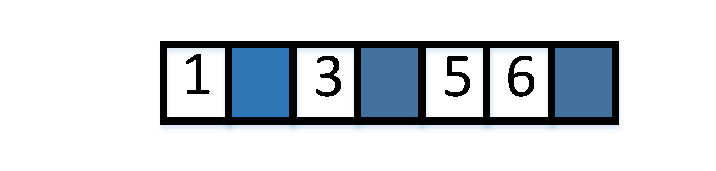
\includegraphics[width=1.6in]{sq1}
\label{sq1}
}
\subfigure[The first rotated subsequence]{
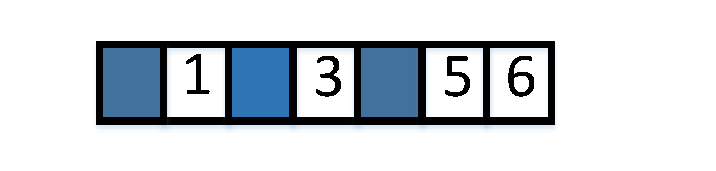
\includegraphics[width=1.6in]{sq2}
\label{sq2}
}
\caption{An example of generated subsequence when $V=\{1,3,5,6\}$, $N=6$ and the first rotated subsequence.}
\label{seq1}
\end{figure}


We then introduce a theorem which will be used in the later discuss.

\begin{theorem}
\label{ro-theo}
Suppose there are two aligned subsequences $S_1$ and $S_2$ with identical length $P$ and $P$ is a prime. Suppose $0 \le k_1 \le P, 0 \le k_2 \le P$ and $k_1 \ne k_2$. If in every period we rotate $S_1$ and $S_2$ to the right by $k_1$ and $k_2$ steps respectively and concatenate them to $S_1$ and $S_2$ respectively. Then after $P$ periods, every element of $S_1$ will meet every element of $S_2$ and vice versa.
\end{theorem}

\begin{figure}[!t]
\centering
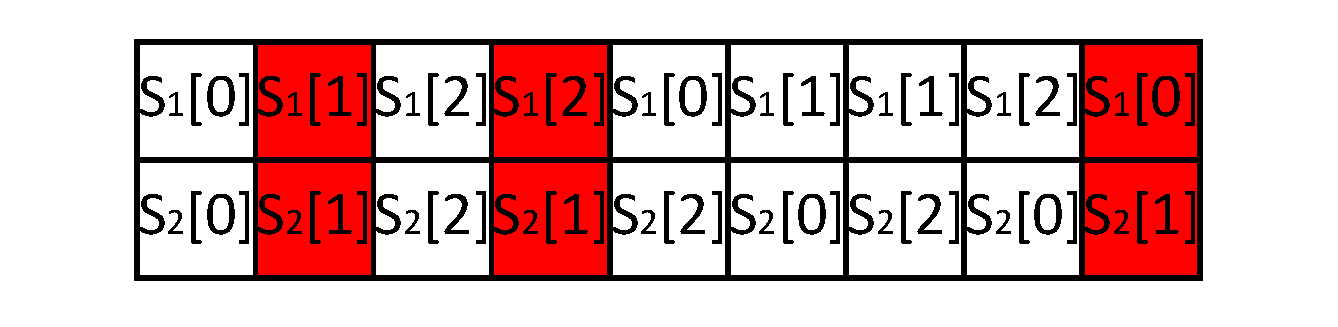
\includegraphics[width=1\columnwidth]{rotate-theo}
\caption{An example of Theorem {\ref{ro-theo}}.}
\label{exp-rotheo}
\end{figure}

\begin{IEEEproof}
Because $S_1$ and $S_2$ are aligned, then $S_1[i]$ will meet $S_2[i]$ in the first period, where $0 \le i < P$. Without lose of generality, suppose $k_1 > k_2$. Let $k_1 - k_2 = m$, then in the later $(P-1)$ periods, $S_1[i]$ will meet $S_2[(i + m)$ mod $P]$, $S_2[(i + 2m)$ mod $P]$, $\cdots$, $S_2[(i+(P-1)m)$ mod $P]$ respectively. According to Theorem \ref{theo}, $i, i + m, i + 2m, \cdots, i + (P-1)m$ are $P$ distinct numbers under modulo-P arithmetic.  Hence, $S_1[i]$ meets all the elements of $S_2$ in $P$ periods and Theorem \ref{ro-theo} holds.
\end{IEEEproof}
Fig.\ref{exp-rotheo} illustrates an example of Theorem {\ref{ro-theo}}, where the length of $S_1$ and $S_2$ is $3$. $S_1$ is rotated to the right by $1$ steps every period, and $S_2$ is rotated to the right by $2$ steps every period. We can clearly see that $S_2[1]$ meets $S_1[1],S_1[2],S_1[0]$ in the three consecutive periods.

\begin{theorem}
\label{theo-alg1}
The MTTR of Alg.\ref{alg1} is $2P^2 + 2P$.
\end{theorem}

\begin{IEEEproof}
We show discuss this problem in two cases.

\bfseries Case 1 \mdseries: Suppose two users choose the same channel, denote it as channel $c$. Without loss of generality, suppose user $i$ starts rendezvous process earlier than user $j$. For clarity, we divide this case into two subcases.

\bfseries Subcase 1.1 \mdseries: Suppose user $j$ starts rendezvous process when user $i$ is still in the first stage, they will both access channel $c$ at the same time. Hence, rendezvous is achieved.

\bfseries Subcase 1.2 \mdseries: Suppose user $j$ starts rendezvous process when user $i$ is already in the second stage. Then in the following $2P$ timeslots, user $i$ will access each available channel including channel $c$ at least once, while user $j$ will stay on channel $c$ in the $2P$ timeslots. Hence, rendezvous can be achieved in the $2P$ timeslots.

\bfseries Case2 \mdseries: Suppose user $i$ and $j$ choose different channels, denote them as channel $(c_i)$ and channel $(c_j)$. When user $i$ and $j$ both get into the second stage, they will both rotate their sequences according to it. There are two situations of periods overlapping of user $i$ and $j$, we will discuss them separately.

\bfseries Subcase 2.1 \mdseries: Suppose the periods of user $i$ and $j$ are aligned, then the scenario is the same as the setting in Theoren \ref{theo} except for that we duplicate the current subsequences before rotate it and attach them to the corresponding sequences. The difference result in double time delay. According to Theorem \ref{ro-theo}, rendezvous will be achieved in $2P^2 + 2P$ timeslots.

\bfseries Subcase 2.2 \mdseries: Suppose the periods of user $i$ and $j$ are not aligned. There are two situations of periods overlapping of user $i$ and $j$ as illustrated in Fig.\ref{sit_period}. The yellow rectangle in Fig.\ref{st1} represents the first half of user $j$'s period, while the red rectangle represents the corresponding part in user $i$'s period. The red rectangle includes all the elements of subsequence $S_i$, because the two halves of user $i$'s period are the same rotated subsequence of $S_i$. Then this situation is similar to Subcase 2.1, and according to Theorem \ref{ro-theo}, rendezvous will be achieved in $2P^2 + 2P$ timeslots. Situation 2 can be analysed in the same way, so we omit it here.

\begin{figure}
\centering
\subfigure[Situation 1]{
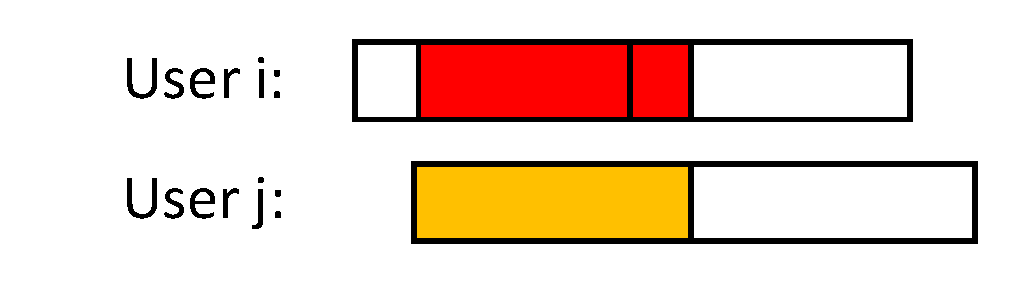
\includegraphics[width=1.6in]{subcasei}
\label{st1}
}
\subfigure[Situation 2]{
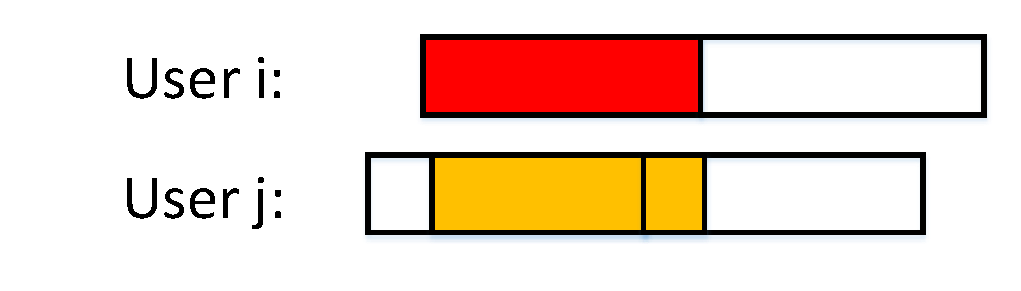
\includegraphics[width=1.6in]{subcaseii}
\label{st2}
}
\caption{Two situations of periods overlapping of user $i$ and $j$}
\label{sit_period}
\end{figure}

Combine these together, we have shown that Theorem \ref{theo-alg1} holds.
\end{IEEEproof}


\begin{theorem}
The RD of Alg.\ref{alg1} is $100\%$ if user $i$ and $j$ choose different channels.
\end{theorem}

\begin{IEEEproof}
If user $i$ and $j$ choose different channels, according to the case 2 of the proof of Theorem \ref{theo-alg1}, every available channel of $V_i$ will meet every available channel of $V_j$ in $2P^2+2P$ timelsots.
\end{IEEEproof}




\section{A Local-Sequence-Based Rendezvous Algorithm Utilizing the ID}
In this section, we will propose an ID-based asynchronous non-anonymous oblivious rendezvous algorithm.



The main idea of this algorithm is to create a channel hopping sequence composed of $l + 1$ subsequences, where $l$ is the length of ID.

\begin{algorithm}
\caption{Local-sequence-based Non-Anonymous Rendezvous Algorithm}
\label{alg3}
\begin{algorithmic}[1]
\STATE Input: the set of available channels $V=\{v_1,v_2,\cdots,v_m\}$, and its binary ID whose length is $l$ bits;
\STATE Find the smallest prime $P$ that ensure $P \ge m$;
\IF{$P = 3$}
\STATE $P:= 5$;
\ENDIF
\STATE Initialize $t := 0, i:= 0, j:= 0$;
\STATE Invoke Alg.\ref{alg2} to generate three sequences $S_1,S_2,S_3$ with channel set V and length $P, P+1, P+2$ respectively;
\STATE Find the channel with the least label in $V$, denote it as channel $(c)$;

\WHILE{Not rendezvous}
\STATE $i := \left \lfloor t / (l+1) \right \rfloor$;
\STATE $j := t $ mod $(l  +1)$;
\IF{$ j < l$}

  \IF{ID$[j] = 0$}
   \STATE Access channel $S_2[i$ mod $(P+1)]$;
    \ELSE
    \STATE Access channel $S_3[i$ mod $ (P+2)]$;
    \ENDIF
\ELSE
\STATE Access channel $S_1[i $ mod $ P]$;
\ENDIF
\STATE $t := t + 1$;
\ENDWHILE

\end{algorithmic}
\end{algorithm}


In Alg.\ref{alg3}, we creates a channel hopping sequence consisting of $(l +1)$ subsequences. The $(l +1)$ subsequences are generated by Alg.\ref{alg2}. There are three kinds of subsequences, which are $S_1, S_2$ and $S_3$. The lengths of $S_1, S_2$ and $S_3$ are P, P+1, P+2 respectively.

Fig.\ref{exp-alg3} illustrates an example of Alg.\ref{alg3}. In this example, the length of ID is 5 and user i's ID is 01101. In round 1, the first $ l$ elements of round 1 are either $S_2[0]$ or $S_3[0]$. If the corresponding digit of the i-th element in ID is 0, then the i-th element will be $S_2[0]$. If the corresponding digit of the i-th element in ID is 1, then the i-th element will be $S_3[1]$. The last element of round 1 is $S_1[0]$.

\begin{theorem}
\label{theo-alg3}
Alg.\ref{alg3} can guarantee rendezvous for two asynchronous users in $(l  + 1)(P_i + 2)(P_j + 2)$ timeslots if $V_i \cap V_j \ne \emptyset$.
\end{theorem}

\begin{figure}[!t]
\centering
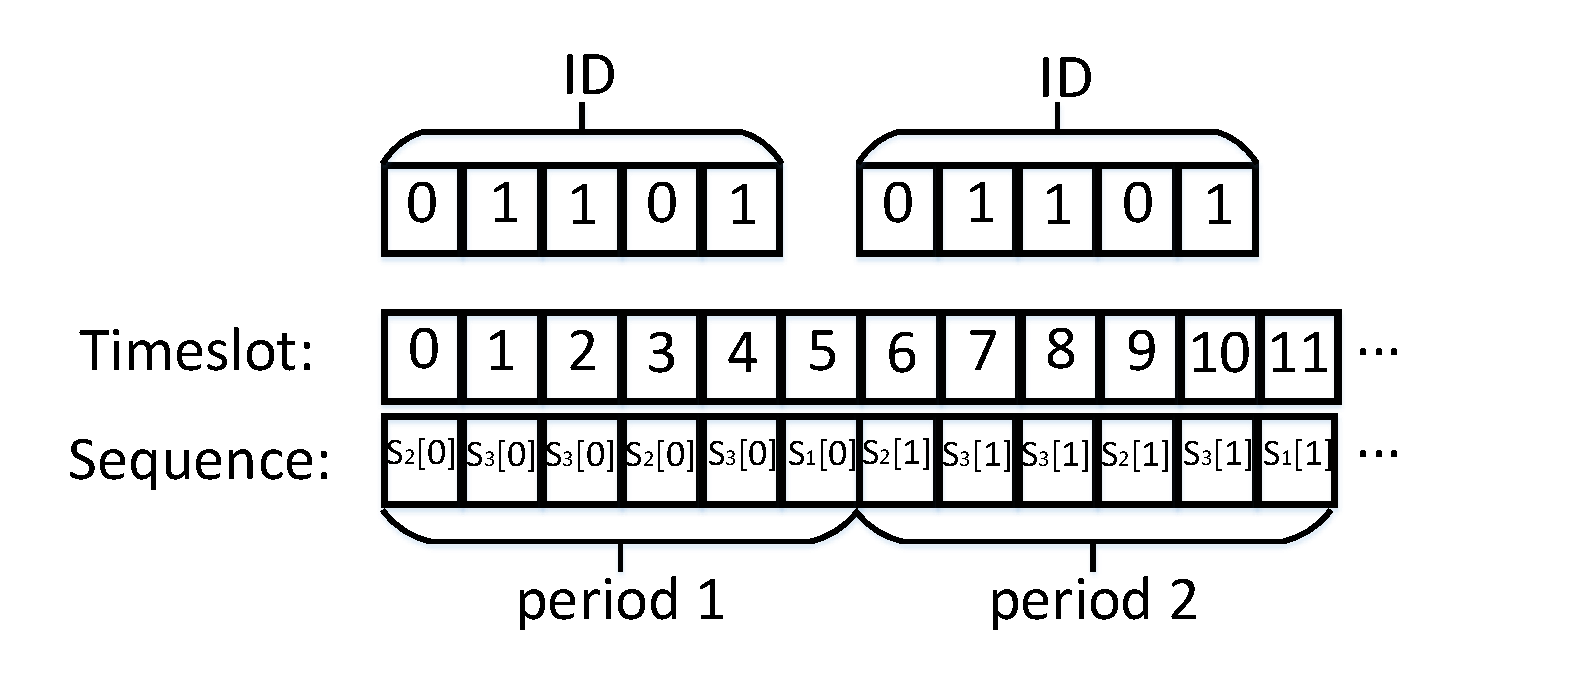
\includegraphics[width=1\columnwidth]{round}
\caption{An example of Alg. {\ref{alg3}}.}
\label{exp-alg3}
\end{figure}


\begin{figure}
\centering
\subfigure[subcase 1]{
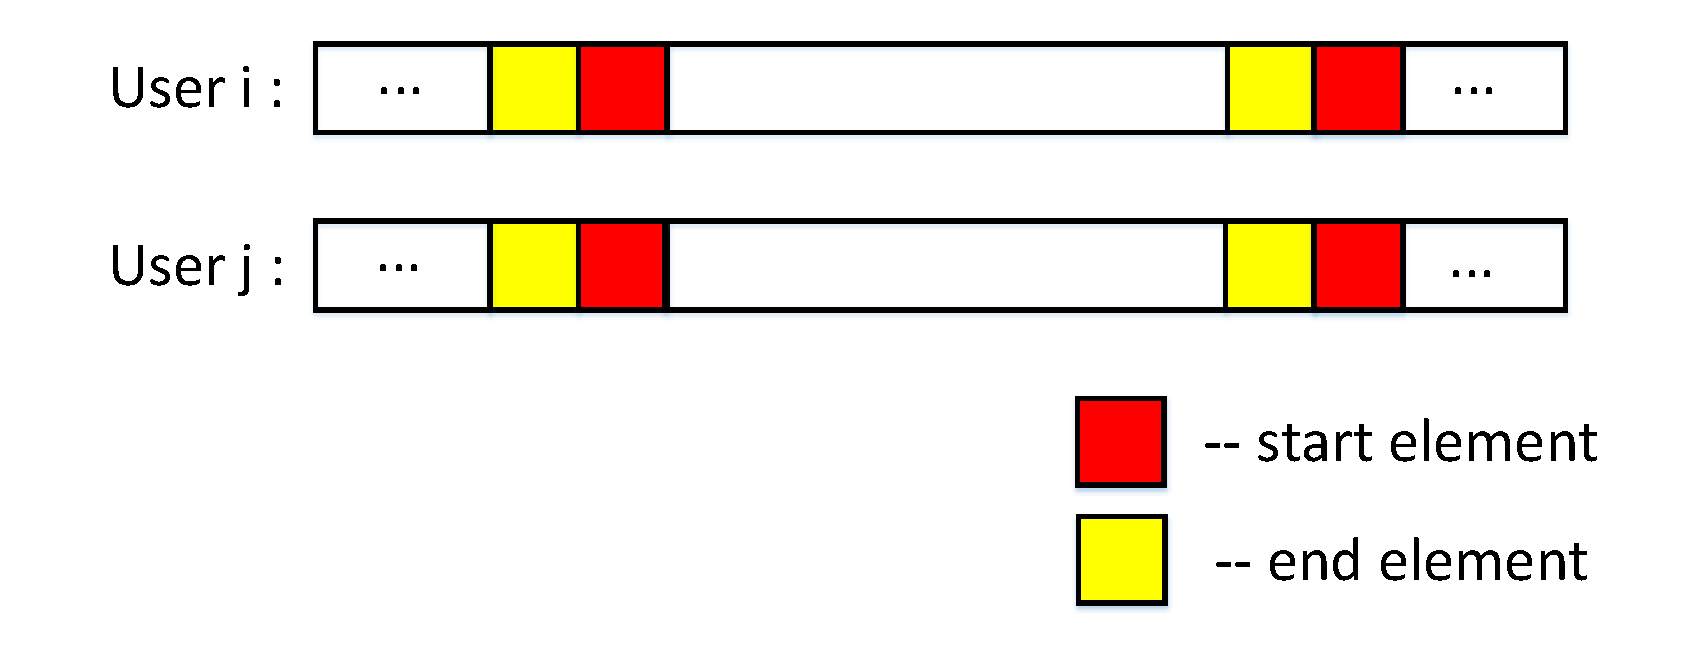
\includegraphics[width=1.6in]{case1}
\label{cs1}
}
\subfigure[subcase 2]{
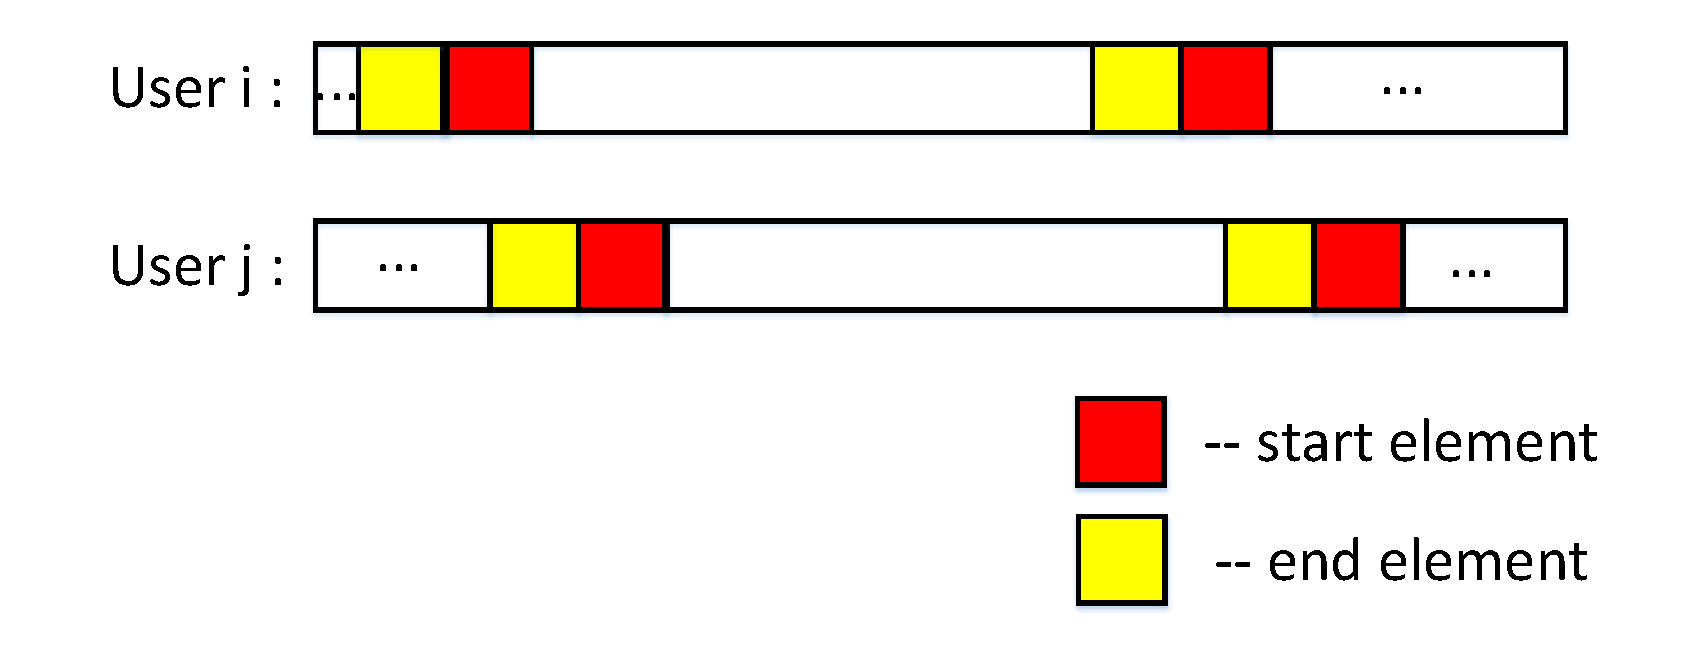
\includegraphics[width=1.6in]{case2}
\label{cs2}
}
\caption{Two subcases of case 1 and case 2.}
\label{case}
\end{figure}



\begin{IEEEproof}
We discuss in two cases:

\bfseries Case 1 \mdseries:

 Suppose $P_i = P_j$. Let $P = P_i =P_j$ We divide this case into two subcases:

\bfseries Subcase 1.1 \mdseries: Suppose user i and j's periods are aligned, as illustrated in Fig.\ref{cs1}. Because user i and user j are two different users, their ID must be different in at least one digit. Without lose of generality, suppose the k-th digit in $ID_i$ is 0 while the k-th digit in $ID_j$ is 1. Then the k-th element in user i's period corresponds to subsequence $S_{2i}$, whose length is $P+1$. The k-th element in user j's period corresponds to subsequence $S_{3j}$, whose length is $P+2$. Then in every period, one element of $S_{2i}$ will meet one element of $S_{2j}$. According to Lemma 2.3, P+1 and P+2 are co-prime. Then rendezvous can be achieved in $(l+ 1)(P+1)(P+2)$ timeslots according to Theorem 2, as long as user i and j have at least one common channel.

\bfseries Subcase 1.2 \mdseries: Suppose user i and j's periods are not aligned, as illustrated in Fig.\ref{cs2}. In this case, the last element in user i's period will meet one of the first $(l + 1)$ elements of user j's period. The last element in user i's period corresponds to subsequence $S_{1i}$. The corresponding element of user j corresponds to subsequence $S_{2j}$ or $S_{3j}$. From Lemma 2.3 and 2.4, we know that P and P+1 are co-prome, P and P +2 are also co-prime. Hence, according to Theorem 2, rendezvous can be achieved in $(l + 1)P(P+1)$ or $(l + 1)P(P+2)$ timeslots respectively.

\bfseries Case 2 \mdseries: Suppose $P_i \ne P_j$.  We divide this case into two subcases:

\bfseries Subcase 2.1 \mdseries: Suppose user i and j's periods are aligned, as illustrated in Fig.\ref{cs1}. In this case, the last
element in user i's period will meet the last element in user j's period. The last element in user i's period corresponds to subsequence $S_{i1}$. The last element in user j's period corresponds to subsequence $S_{j1}$. Because $P_i \ne P_j$, rendezvous can be achieved in $(l + 1)P_iP_j$ timeslots according to Theorem 2, as long as user i and j have at least one common channel.

\bfseries Subcase 2.2 \mdseries: Suppose user i and j's periods are not aligned, as illustrated in Fig.\ref{cs2}. Without lose of generality, suppose $P_i > P_j$. In this case, the last element in user i's period will meet one of the first $(l + 1)$ elements of user j's period. The last element in user j's period will meet one of the first $(l + 1)$ elements of user i's period. The last element in user j's period corresponds to subsequence $S_{1j}$, whose length is $P_j$. The corresponding element of user j corresponds to subsequence $S_{2i}$ or $S_{3i}$, whose lengths are $P_i +1$ and $P_i +2$ respectively. Because $P_i$ and $P_j$ are two different primes, $P_i > P_j +2$ or $P_i = P_j +2$. If $P_i > P_j + 2$, from Lemma 2.5, we know $P_i$ and $P_j + 1$ are co-prime, $P_i$ and $P_j +2 $ are co-prime. According to Theorem 2, rendezvous can be achieved in $(l + 1)P_i(P_j+1)$ or $(l + 1)P_i(P_j+2)$ timeslots respectively. If $P_i = P_j + 2$, then $P_i + 1 = P_2 + 3$, $P_i + 2 = P_j + 4$. If $P_j = 2$, $P_i = 2 + 2=4$ is not a prime. In Alg.\ref{alg3}, we set P to be 5 if $P=3$. Because $P_2 \ne 2$ and $P_2 \ne 3$, $P_2 + 3$ and $P_2 + 4$ can not be divided by $P_2$ without remainder. From Lemma 2.5, we know that both $P_i + 1$ and $P_i +2$ are co-prime with $P_j$. According to Theorem 2, rendezvous can be achieved in $(l + 1)(P_i + 1)P_j$ or $(l + 1)(P_i+2)P_j$ timeslots respectively.

Combine the above together, Theorem \ref{theo-alg3} holds.

\end{IEEEproof}

\begin{theorem}
\label{theo-rd-alg3}
The RD of Alg.\ref{alg3} is 100\%.
\end{theorem}

\begin{IEEEproof}
For any user, the corresponding subsequence $S_1,S_2,S_3$ all contains all the channels in its available channel set. From the proof of Theorem 3, we know that one subsequence of user $i$ will meet one subsequence of user $j$ and the lengths of the subsequences are co-prime. Denote the two subsequences as $S_i$ and $S_j$. From Theorem \ref{theo}, we know that every element in $S_i$ will meet all of the elements in $S_j$ and vice versa. Hence, the RD of Alg.\ref{alg3} is 100\%.
\end{IEEEproof}

\section{A Local-Sequence-Based Rendezvous Algorithm Utilizing the Channel Label}
In this section, we will propose a rendezvous algorithm which utilizes the label of a channel in the available channel set.
\begin{algorithm}
\caption{Channel-Label-Based Local-sequence-based Non-Oblivious Rendezvous Algorithm}
\label{alg4}
\begin{algorithmic}[1]
\STATE Input: the set of available channels $V=\{v_1,v_2,\cdots,v_m\}$ and the number of all channels: $N$;

\STATE Find the smallest prime $P$ that ensure $P \ge m$;
\IF{$P = 3$}
\STATE $P := 5$;
\ENDIF
\STATE Randomly choose a channel $c$ from $V$;
\STATE Convert $c$ into a binary string $CH$ whose length is $\left \lceil log_2 N \right \rceil$;

\STATE Invoke Alg.\ref{alg2} to generate three subsequences $S_1, S_2, S_3$ with channel set $V$ and length $P, P+1, P+2$ respectively.

\STATE Initialize $t := 0$, $i := 0$, $j:=0$;
\WHILE{Not rendezvous}
\IF{$ t < P_N(\left \lceil log_2 N \right \rceil +1)$}
\STATE Access channel $(c)$;
\ELSE
 \STATE $i := \left \lfloor t / ((\left \lceil log_2 N \right \rceil +1)) \right \rfloor$;
 \STATE $j :=  t$ mod $ (\left \lceil log_2 N \right \rceil + 1)$;
  \IF{$ j < \left \lceil log_2 N \right \rceil$}
    \IF{$CH[j] = 0$}
     \STATE Access channel $S_2[i $ mod $ (P+1)]$;
      \ELSE
     \STATE Access channel $S_3[i $ mod $ (P+2)]$;
     \ENDIF
  \ELSE
\STATE Access channel $S_1[i $ mod $ P]$;
\ENDIF
\ENDIF
\STATE $t:=t+1$;
\ENDWHILE
\end{algorithmic}
\end{algorithm}

The main idea of Alg.\ref{alg4} is to randomly choose an available channel $c$ from $V$ and use the binary representation of $c$ as the user's ID. It is obvious that the available channel chosen by two users can be identical, but our algorithm can solve this problem, because the label of an available channel is very useful.



In Alg.\ref{alg4}, we divide timeslots into two subsequences, $S$ and $C$. Subsequence $S$ is further divided into three subsequences $S_1,S_2$ and $S_3$. Subsequence $C$ is filled with channel ($c$). There are three situations of the overlapping of the timeslots of user $i$ and $j$, as shown in Fig.\ref{sit-alg4}

\begin{figure}
\centering
\subfigure[Situation 1]{
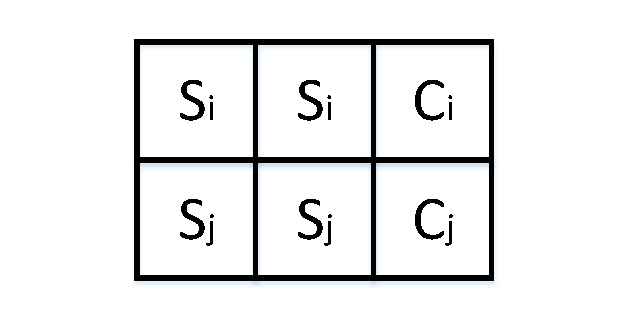
\includegraphics[width=0.8in]{situation1}
\label{stu1}
}
\subfigure[Situation 2]{
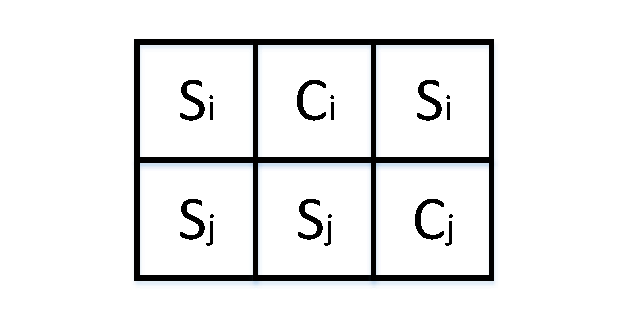
\includegraphics[width=0.8in]{situation2}
\label{stu2}
}
\subfigure[Situation 3]{
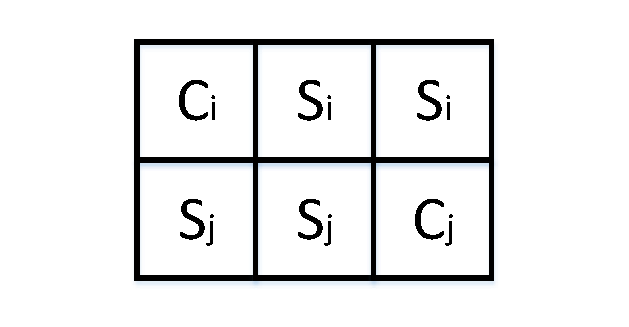
\includegraphics[width=0.8in]{situation3}
\label{stu3}
}
\caption{Three situations of timeslot overlapping of user $i$ and $j$.}
\label{sit-alg4}
\end{figure}

\begin{theorem}
\label{theo-alg4}
Alg. \ref{alg4} can guarantee rendezvous for two asynchronous users in $3(P_i+2)(P_j+2)(\left \lceil log_2N \right \rceil +1)$ timeslots as long as $V_i \cap V_j \ne \emptyset$.
\end{theorem}

\begin{IEEEproof}
We discuss this problem in two cases.

\bfseries Case 1: \mdseries Suppose the overlapping of timeslots of user $i$ and user $j$ is as shown in Fig.\ref{stu1}. Then we discuss in two subcases.

\bfseries Subcase 1.1: \mdseries If two users choose the same channel, because $C_i$ meets $C_j$ every period and $c_i =c_j$, rendezvous will be achieved in one period, which is $3$ timeslots.

\bfseries Subcase 1.2: \mdseries If two users choose different channels, then $CH_i$ will be different from $CH_j$ in at least one bit. Then this situation is the same as that in Alg.\ref{alg3}, except for the time cost is three times. According to the proof of Theorem \ref{theo-alg3}, rendezvous for user $i$ and user $j$ will be achieved in  $3(P_i+2)(P_j+2)(\left \lceil log_2N \right \rceil +1)$ timeslots.

\bfseries Case 2: \mdseries Suppose the overlapping of timeslots of user $i$ and user $j$ is as shown in Fig.\ref{stu2} or Fig.\ref{stu3}.
We also discuss in two subcases.

\bfseries Subcase 2.1: \mdseries If two users choose the same channel, denote it as channel ($c$). Then channel ($c$) is in both $S_{ki} (k = 1,2,3)$ and $S_{kj} (k = 1,2,3)$. Because $S_i$ overlaps with $C_j$ and $S_j$ overlaps with $C_i$ in every period, then $C_j$ will meet all the elements of $S_{1i}$ in $(\left \lceil log_2N \right \rceil +1)P_j$ periods, which are $3(\left \lceil log_2N \right \rceil +1)P_j$ timeslots. Hence, rendezvous will be achieved in $3(\left \lceil log_2N \right \rceil +1)P_j$ timeslots.

\bfseries Subcase 2.2: \mdseries If two users choose different channels, then $CH_i$ will be different from $CH_j$ in at least one bit. Because in both Fig.\ref{stu2} and Fig.\ref{stu3}, $S_i$ overlaps with $S_j$, this situation is the same as that in Alg.\ref{alg3}, except for the time cost is three times. According to the proof of Theorem \ref{theo-alg3}, rendezvous for user $i$ and user $j$ will be achieved in  $3(P_i+2)(P_j+2)(\left \lceil log_2N \right \rceil +1)$ timeslots.

Combine these together, Theorem \ref{theo-alg4} holds.
\end{IEEEproof}

\begin{theorem}
The RD of Alg.\ref{alg4} is $100\%$ if user $i$ and $j$ choose different channels.
\end{theorem}

\begin{IEEEproof}
If user $i$ and $j$ choose different channels, then $CH_i$ and $CH_j$ are two different strings. Because $S_i$ overlaps with $S_j$ in all cases, the situation is the same as that in Alg.\ref{alg3}. From the proof of Theorem \ref{theo-rd-alg3}, we know that the RD of Alg.\ref{alg4} is $100\%$.
\end{IEEEproof}

\section{Simulation}

\section{Conclusion}

\section{Acknowledgements}



%\bibliographystyle{plain}
%\bibliography{references}
\end{document}


